\documentclass{llncs}
\usepackage{xspace}
\usepackage{amssymb}
\usepackage{wrapfig}
\usepackage{paralist}
% \usepackage{multirow}
% \usepackage{multicol}
\usepackage{url}
\usepackage{lstomdoc}\lstset{language=[1.3]OMDoc,columns=fullflexible,basicstyle=\sf}
%\usepackage{stex-logo}
\def\stex{\texorpdfstring{\raisebox{-.5ex}S\kern-.5ex\TeX}{sTeX}}
\def\sTeX{\stex}

\usepackage{rotating}
\usepackage{tikz}
\usetikzlibrary{arrows}
%\usepackage[today,eso-foot]{svninfo}
\usepackage[final]{svninfo}

\svnInfo $Id: paper.tex 9200 2012-04-20 20:37:20Z frabe $
\svnKeyword $HeadURL: https://svn.omdoc.org/repos/omdoc/projects/omdoc-2.0/pragmatic-strict/paper.tex $

\setcounter{tocdepth}{2} % for pdf bookmarks
\usepackage[bookmarks,linkcolor=red,citecolor=blue,urlcolor=gray,colorlinks,breaklinks,bookmarksopen,bookmarksnumbered]{hyperref}

\usepackage{twelf-math}
\usepackage{basics}
\usepackage{pattern}
\usepackage{local}
%\usepackage{reltable}
%\usepackage{ded}
%\usepackage{mmt_new}

\title{Extending MKM Formats at the Statement Level}
\author{Fulya Horozal, Michael Kohlhase, and Florian Rabe}
\authorrunning{Horozal, Kohlhase, Rabe}
\institute{
\begin{tabular}[t]{c}
  Computer Science, Jacobs University Bremen, Germany
  \url{http://kwarc.info}
\end{tabular}
}
\begin{document}
\maketitle
\begin{abstract}
  Successful representation and markup languages find a good balance between giving the
  user freedom of expression, enforcing the fundamental semantic invariants of the
  modeling framework, and allowing machine support for the underlying semantic
  structures. MKM formats maintain strong invariants while trying to be foundationally
  unconstrained, which makes the induced design problem particularly challenging.

  In this situation, it is standard practice to define a minimal core language together
  with a scripting/macro facility for syntactic extensions that map into the core
  language. In practice, such extension facilities are either fully unconstrained (making
  invariants and machine support difficult) or limited to the object level (keeping the
  statement and theory levels fixed). 

  In this paper we develop a general methodology for extending MKM representation formats
  at the statement level. We show the utility (and indeed necessity) of statement-level
  extension by redesigning the \omdoc format into a minimal, regular core language (strict
  \omdoc) and an extension (pragmatic \omdoc) that maps into strict \omdoc.
\end{abstract}

\section{Introduction}\label{sec:intro}
 \svnInfo $Id: intro.tex 9171 2012-03-05 08:39:33Z kohlhase $
\svnKeyword $HeadURL: https://svn.omdoc.org/repos/omdoc/projects/omdoc-2.0/pragmatic-strict/intro.tex $

The development of representation languages for mathematical knowledge is one of the
central concerns of the MKM community. After all, practical mathematical knowledge
management consists in the manipulation of expressions in such languages. To be
successful, MKM representation formats must balance multiple concerns. A format should be
expressive and flexible (for depth and ease of modeling), foundationally unconstrained
(for coverage), regular and minimal (for ease of implementation), and modular and
web-transparent (for scalability). Finally, the format should be elegant, feel natural to
mathematicians, and be easy to read and write. Needless to say that this set of
requirements is over-constrained so that the design problem for MKM representation formats
lies in relaxing some of the constraints to achieve a global optimum.

In languages for formalized mathematics, it is standard practice to define a minimal
core language that is extended by macros, functions, or notations.
For example, Isabelle \cite{isabelle} provides a rich language of notations, abbreviations, syntax and printing translations, and a number of definitional forms.
In narrative formats for mathematics, for
instance, the {\TeX/\LaTeX} format -- arguably the most commonly used format for
representing mathematical knowledge -- goes a similar way, only that the core language is
given by the {\TeX} layout primitives and the translation is realized by macro expansion
and is fully under user control. This extensibility led to the profusion of
user-defined {\LaTeX} document classes and packages that has made {\TeX/\LaTeX} so
successful.

However, the fully unconstrained nature of the extensibility makes ensuring invariants and
machine support very difficult, and thus this approach is not immediately applicable to
content markup formats. There, MathML3~\cite{CarlisleEd:MathML3:base} is a good example of
the state of the art. It specifies a core language called ``strict content MathML'' that
is equivalent to OpenMath~\cite{BusCapCar:2oms04} and ``full content MathML''. The first
subset uses a minimal set of elements representing the meaning of a mathematical
expression in a uniform, regular structure, while the second one tries to strike a
pragmatic balance between verbosity and formality. The meaning of non-strict expressions
is given by a fixed translation: the ``strict content MathML translation'' specified in
section 4.6 of the MathML3 recommendation~\cite{CarlisleEd:MathML3:base}.

This language design has the advantage that only a small, regular sublanguage has to be
given a mathematical meaning, but a larger vocabulary that is more intuitive to
practitioners of the field can be used for actual representation. Moreover, semantic
services like validation only need to be implemented for the strict subset and can be
extended to the pragmatic language by translation. Ultimately, a representation format
might even have multiple pragmatic front-ends geared towards different audiences. These
are semantically interoperable by construction.
\medskip

The work reported in this paper comes from an ongoing language design effort, where we
want to redesign our \omdoc format~\cite{Kohlhase:OMDoc1.2} into a minimal, regular core
language (\emph{strict \omdoc2}) and an extension layer (\emph{pragmatic \omdoc2}) whose
semantics is given by a ``pragmatic-to-strict'' ($\ptos$) translation.  While this problem
is well-understood for mathematical \emph{objects}, extension frameworks \emph{at the
  statement level} seem to be restricted to the non-semantic case, e.g. the
\texttt{amsthm} package for {\LaTeX}.

Languages for mathematics commonly permit a variety of pragmatic statements, e.g.,
implicit or case-based definitions, type definitions, theorems, or proof schemata.  But
representation frameworks for such languages do not include a generic mechanism that
permits introducing arbitrary pragmatic statements --- instead, a fixed set is built into
the format.  Among logical frameworks, Twelf/LF~\cite{twelf,lf} permits two statements:
defined and undefined constants. Isabelle~\cite{isabelle} and Coq~\cite{coq} permit much
larger, but still fixed sets that include, for example, recursive case-based function
definitions.  Content markup formats like \omdoc permit similar fixed sets.

A large set of statements is desirable in a representation format in order to model the
flexibility of individual languages. A large \emph{fixed} set on the other hand is
unsatisfactory because it is difficult to give a theoretical justification for fixing any
specific set of statements.  Moreover, it is often difficult to define the semantics of a
built-in statement in a foundationally unconstrained representation format because many
pragmatic statement are only meaningful under certain foundational assumptions.
%For example, an existential quantifier is needed to express the well-definedness condition of an implicit definition.
\medskip

In this paper we present a general formalism for adding new pragmatic statement forms to
our \omdoc format; we have picked \omdoc for familiarity and foundation-independence; any
other foundational format can be extended similarly. Consider for instance the pragmatic
statement of an ``implicit definition'', which defines a mathematical object by describing
it so accurately, that there is only one object that fits this description. For instance,
the exponential function $exp$ is defined as the (unique) solution of the differential
equation $f=f'$ with $f(0)=1$. This form of definition is extensively used in practical
mathematics, so pragmatic {\omdoc} should offer an infrastructure for it, whereas strict
{\omdoc} only offers ``simple definitions'' of the form $c:=d$, where $c$ is a new symbol
and $d$ any object.  In our extension framework, the $\ptos$ translation provides the
semantics of the implicit definition in terms of the strict definition $exp:=\descr
f.(f'=f\wedge f(0)=1)$, where $\descr$ is a ``definite description operator'': Given an
expression $A$ with free variable $x$, such that there is a unique $x$ that makes $A$
valid, $\descr x.A$ returns that $x$, otherwise $\descr x.A$ is undefined.

Note that the semantics of an implicit definition requires a definite description operator.
While most areas of mathematics at least implicitly assume its existence, it should not be required in general because that would prevent the representation of systems without one.
Therefore, we make these requirements explicit in a special theory that defines the new pragmatic statement and its strict semantics. This theory must be imported in order for implicit definitions to become available.
Using our extension language, we can recover a large number of existing pragmatic statements as definable special cases, including many existing ones of {\omdoc}.
Thus, when representing formal languages in {\omdoc}, authors have full control what pragmatic statements to permit and can define new ones in terms of existing ones.
\medskip

In the next section, we will recap those parts of \omdoc that are
needed in this paper. In Section~\ref{sec:pattern}, 
we define our extension language, and in Section~\ref{sec:meta}, we look at particular extensions that are motivated by mathematical practice. Finally, in Section~\ref{sec:syntax}, we will address the question
of extending the concrete syntax with pragmatic features as well.



%%% Local Variables: 
%%% mode: latex
%%% TeX-master: "paper"
%%% End: 

% LocalWords:  wrapfigure vspace hline ednote emph emph RabKoh prel Rudnicki lf
% LocalWords:  isabelle-isar aomp92 omdoc ptos frabe medskip texttt amsthm exp
% LocalWords:  descr

 %\svnInfo $Id: features.tex 9179 2012-03-14 20:20:33Z fhorozal $
\svnKeyword $HeadURL: https://svn.omdoc.org/repos/omdoc/projects/omdoc-2.0/pragmatic-strict/features.tex $
\section{Generic Elaboration of Pragmatic Language Features}
 A \defemph{feature} consists of three components:
\begin{itemize}
  \item an {\mmt} theory, called the \defemph{feature theory},
  \item an extension of the {\mmt} grammar and type system with symbol-level declarations, called the \defemph{feature-dependent syntax},
  \item an \defemph{elaboration} of the feature-dependent syntax into {\mmt} syntax
\end{itemize}

We will abbreviate the URI \url{http://cds.omdoc.org/features} with $\cn{Feat}$.

\paragraph{Logic}
The feature of being a logic is defined as follows.
The feature theory is given by
\[\thdecl{\feath{Logic}}{\symdd{o}{}{},\;\symdd{ded}{}{}}\]
The pragmatic syntax is given by
\[Sym \;\bnfas\; \mmtaxiom{a}{F}\]
The well-formedness rule is
\[\ianc{\otermtype{\TG}{\qT}{F}{o}}
       {\osym{\TG}{\qT}{\mmtaxiom{a}{F}}}
       {}\]
\ednote{Alternatively, the semantics can be defined through elaboration. Then this would become a theorem.}

The elaboration is given by
\[\elaborate{\mmtaxiom{a}{F}}
            {\symdd{a}{\oma{ded,F}}}{}\]
\ednote{ded here actually refers to the meaning of ded within $\qT$. This must be
  discussed.}
%%% Local Variables: 
%%% mode: latex
%%% TeX-master: "paper"
%%% End: 

% LocalWords:  defemph mmt cn thdecl feath symdd symdd ded Sym bnfas mmtaxiom
% LocalWords:  ianc otermtype osym ednote

  
  
\section{MMT/OMDoc}\label{sec:mmt}
 \svnInfo $Id: mmt.tex 9195 2012-04-20 12:26:50Z frabe $
\svnKeyword $HeadURL: https://svn.omdoc.org/repos/omdoc/projects/omdoc-2.0/pragmatic-strict/mmt.tex $

\begin{wrapfigure}r{3.2cm}\vspace*{-2em}
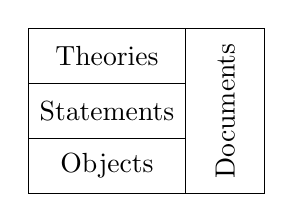
\begin{tikzpicture}[yscale=.7]
\draw (0,0) rectangle (3,3);
\draw (0,1) -- (2,1);
\draw (0,2) -- (2,2);
\draw (2,0) -- (2,3);
\node (thy) at (1,2.5) {Theories};
\node (st) at (1,1.5) {Statements};
\node (obj) at (1,0.5) {Objects};
\node (doc) at (2.5,1.5){\begin{sideways}Documents\end{sideways}};
\end{tikzpicture}
\vspace*{-2em}
\end{wrapfigure}
\omdoc is a comprehensive content-based format for representing mathematical knowledge and
documents. It represents mathematical knowledge at three levels: mathematical formulae at the
\emph{object level}, symbol declarations, definitions, notation definitions, axioms, theorems, and
proofs at the \emph{statement level}, and finally modular scopes at the \emph{theory level}. Moreover, it adds
an infrastructure for representing functional aspects of \emph{mathematical documents} at the
content markup level. \omdoc1.2 has been successfully used as a representational basis in applications
ranging from theorem prover interfaces, via knowledge based up to eLearning systems. To allow
this diversity of applications, the format has acquired a large, interconnected set of language
constructs motivated by coverage and user familiarity (i.e., by pragmatic concerns) and not by
minimality and orthogonality of language primitives (strict concerns).

To reconcile these language design issues for \omdoc2, we want to separate the format into a \emph{strict} core language
and a \emph{pragmatic} extension layer that is elaborated into strict \omdoc via a ``pragmatic-to-strict'' ($\ptos$) translation.

For strict \omdoc we employ the foundation-independent, syntactically minimal {\mmt} framework
(see below). For pragmatic \omdoc, we aim at a language that is feature-complete with
respect to \omdoc1.2~\cite{Kohlhase:OMDoc1.2}, but incorporates language features from
other MKM formats, most notably from Isabelle/Isar~\cite{isar},
PVS~\cite{pvs}, and Mizar~\cite{mizar}.

The {\mmt} language was emerged from a complete redesign of the formal core\footnote{We are currently
  working on adding an informal (natural language) representation and a non-trivial (strict)
  document level to {\mmt}, their lack does not restrict the results reported in this paper.} of \omdoc
focusing on foundation-independence, scalability, modularity, while maintaining coverage of formal
systems. The {\mmt} language is described in~\cite{RK:mmt:10} and implemented
in~\cite{project:mmt}.

\begin{wrapfigure}{l}{5.2cm}\vspace*{-2em}
\begin{center}
\begin{tikzpicture}[xscale=.95,yscale=.7]
\node[thy] (A) at (0,3)  {$\mathit{LF}$};
\node[thy] (A') at (2,3)  {$\mathit{Isabelle}$};
\node[thy] (C) at (-1,1.5)   {$\mathit{FOL}$};
\node[thy] (C') at (1,1.5) {$\mathit{HOL}$};
\node[thy] (E) at (-2,0) {$\mathit{Monoid}$};
\node[thy] (E') at (0,0)  {$\mathit{Ring}$};
\draw[meta](A) -- (C);
\draw[meta](A) -- (C');
\draw[meta](C) -- (E);
\draw[meta](C) -- (E');
\draw[struct](A) --node[above] {} (A');
\draw[struct](C) --node[above] {} (C');
\draw[struct](E) --node[above] {} (E');
%\draw[struct](A) --node[above] {$m$} (A');
%\draw[struct](C) --node[above] {$m'$} (C');
%\draw[struct](E) --node[above] {$i$} (E');
\end{tikzpicture}
\caption{An {\mmt} Theory Graph}\label{fig:mmt:intro:metatheory}
\end{center}\vspace*{-2em}
\end{wrapfigure}

MMT uses \defemph{theories} as a single primitive to represent formal systems such as logical frameworks, logics, or theories.
These form theory graphs such as the one on the left, where single arrows $\rightarrow$ denote theory translations and hooked arrows $\hookrightarrow$ denote the meta-theory relation between two theories.
The theory $\mathit{FOL}$ for first-order logic is the meta-theory for $\mathit{Monoid}$ and $\mathit{Ring}$. And the theory $\mathit{LF}$
for the logical framework LF~\cite{lf} is the meta-theory of $\mathit{FOL}$ and $\mathit{HOL}$ for higher-order logic.
In general, we describe the theories with meta-theory $M$ as \defemph{$M$-theories}.
The importance of meta-theories in {\mmt} is that the syntax and semantics of $M$ induces the syntax and semantics of all $M$-theories.
For example, if the syntax and semantics are fixed for $\mathit{LF}$, they determine those of $\mathit{FOL}$ and $\mathit{Monoid}$.

At the statement level, {\mmt} uses \defemph{constant} declarations as a single primitive to represent all OMDoc statement declarations. These are differentiated by the type system of the respective meta-theory. In particular, the Curry-Howard correspondence is used to represent axioms and theorems as plain constants (with special types).
\medskip

In Figure~\ref{fig:mmt-grammar}, we show a small fragment of the {\mmt} grammar that we need in the remainder of this paper. Meta-symbols of the BNF format are given in \bnf{color}.
%the salient language features layered according the \omdoc stratification.

%{\mmt} is meant to be applicable to all base languages based on \emph{theories}. Relations between theories (theory morphisms) are represented as {\mmt} \emph{views}. Both theories and views form the {\mmt} \emph{theory} level. A \emph{theory morphism} $\overline{\sigma} : S \rightarrow T$ is a \emph{signature morphism} $\sigma : S \rightarrow T$ interpreting all symbols of $S$ in $T$ and, in addition, $\overline{\sigma}$ translates all theorems of $S$ to theorems of $T$. {\mmt} uses the \emph{Curry-Howard representation} to drop the distinction between symbols and axioms (and thus between signatures and theories). As a result, {\mmt} needs only theories and theory morphisms.

\begin{figure}[ht]
\begin{center}
\begin{tabular}{|@{\hspace{.4em}}l@{\tb}l@{\hspace{.4em}}l@{\hspace{.4em}}l@{\hspace{.4em}}|}
\hline
Modules              & $G$      &$\bnfas$& $\bnf{(}\lfkw{theory}\;\,T = \{\Sigma\}\bnf{)^{\ast}}$\\
Theories             & $\Sigma$ &$\bnfas$& $\cdot\bnfalts\Sigma,\,%\lfkw{constant}\;\,
c \bnf{[}:E \bnf{][}=E\bnf{]}\bnfalts \lfkw{meta}\;\,T$\\   
Contexts     & $\Gamma$ &$\bnfas$& $\cdot\bnfalts\Gamma,\,x\bnf{[}:E\bnf{]}$\\ 
Expressions          & $E$      &$\bnfas$& $x\bnfalts c\bnfalts E\,E^{\bnf{+}}\bnfalts E\,\Gamma.\,E$ \\
\hline
\end{tabular}
\end{center}
\caption{{\mmt} Grammar}\label{fig:mmt-grammar}
\end{figure}

The module level of {\mmt} introduces \emph{theory declarations} $\lfkw{theory}\;\,T = \{\Sigma\}$. %\stackrel{M}{=}
Theories $\Sigma$ contain \emph{constant declarations} $c[:E_1][=E_2]$ that introduce named atomic expressions $c$ with optional type $E_1$ or definition $E_2$. Moreover, %theories can include other theories $T$ via $\lfkw{include}\;T$, and 
each theory may declare its meta-theory $T$ via $\lfkw{meta}\;T$.

{\mmt} expressions are a fragment of OpenMath~\cite{openmath} objects, for which we introduce a short syntax. They are formed from variables $x$, constants $c$, applications $E\,E_1\,\ldots\, E_n$ of functions $E$ to a sequence of arguments $E_i$, and bindings $E_1\,\Gamma.\,E_2$ that use a binder $E_1$, a context $\Gamma$ of bound variables, and a scope $E_2$.
Contexts $\Gamma$ consist of variables $x[:E]$ that can optionally attribute a type $E$.

The semantics of {\mmt} is given in terms of \emph{foundations} for the upper-most meta-theories. Foundations define in particular the typing relation between expressions, in which {\mmt} is parametric.
For example, the foundation for $\mathit{LF}$ induces the type-checking relation for all theories with meta-theory $\mathit{LF}$.

\begin{example}[{\mmt}-Theories]Below we give an {\mmt} theory $\Forms$, which will serve as the meta-theory of several logics introduced in this paper. It introduces all symbols needed to declare logical connectives and inference rules of a logic.
The syntax and semantics of this theory are defined in terms of type theory, e.g., the logical framework LF \cite{lf}.

\begin{tabular}{@{\hspace{-.55cm}}l@{\hspace{1cm}}l}
\begin{minipage}[b]{7cm}
$\kity$, $\rightarrow$, and $\lmbd$ are untyped constants representing the primitives of type theory. $\kity$ represents the universe of all types, $\rightarrow$ constructs function types $\alpha\to\beta$, and $\lmbd$ represents the $\lambda$-binder.
$\form$ is the type of logical formulas and  
%a typed constant representing the set of logical formulas. 
$\ded$ is a constant that assigns to each logical formula $F:\form$ the type $\ded\,F$ of its proof. 
\end{minipage} &
\begin{minipage}[b]{4cm}
\begin{twelfsig}
\tsig{\Forms}\\
$\kity$\\
$\rightarrow$\\
$\lmbd$\\
\decl{\form}{\kity}\\
\decl{\ded}{\form\to\kity}\\
\tsigend
\end{twelfsig}
\end{minipage}
\end{tabular}
\end{example}


%\begin{wrapfigure}{r}{4cm}
%\vspace{-3em}
%\begin{center}
%\begin{twelfsig}
%\tsig{\Forms}\\
%$\kity$\\
%$\rightarrow$\\
%$\lmbd$\\
%\decl{\form}{\kity}\\
%\decl{\ded}{\form\to\kity}\\
%\tsigend
%\end{twelfsig}
%\end{center}
%\vspace{-5em}
%\caption{An Example {\mmt} Theory}\label{fig:ex-mmt}
%\end{wrapfigure}

%{\mmt} theories consist of \emph{symbol declarations}. 
%{\mmt} views consist of \emph{symbol assignments}.  
%\emph{Constants} represent declarations of the base language.
%\emph{Structures} represent inheritance between theories.  
%\emph{Constant assignments} and \emph{structure assignments} represent assignments between constants and structures respectively. \emph{Links} are an {\mmt} module level notion that generalizes both structures and views. 
%Symbol declarations and assignments form a {\mmt} symbol level.  
%\emph{Terms} appear inside {\mmt} constants (e.g. as type or definition) and their grammar is motivated by the OpenMath grammar. They form the {\mmt} object level.


%%% Local Variables: 
%%% mode: latex
%%% TeX-master: "paper"
%%% End: 

% LocalWords:  mmt.tex wrapfigure vspace tikzpicture yscale omdoc emph Rudnicki
% LocalWords:  isabelle-isar aomp92 ednote RabKoh mmt-ontology overline hspace
% LocalWords:  rightarrow rightarrow ysep theo-name symb-name 5.2truecm xscale
% LocalWords:  cn mmt defemph frabe ptos pvs mathit hookrightarrow lf medskip
% LocalWords:  bnf hline bnfas lfkw cdot bnfalts stackrel ldots kity lmbd kity
% LocalWords:  ded ded twelfsig tsig tsigend

  
\section{A Framework for Language Extensions}\label{sec:pattern}  
 \svnInfo $Id: pattern.tex 9195 2012-04-20 12:26:50Z frabe $
\svnKeyword $HeadURL: https://svn.omdoc.org/repos/omdoc/projects/omdoc-2.0/pragmatic-strict/pattern.tex $

We will now define our extension language (EL). It provides a syntactic means to define pragmatic language features and their semantics in terms of strict {\omdoc}.

\paragraph{Syntax}
EL adds two primitive declarations to {\mmt} theories: \emph{extension declarations} and \emph{pragmatic declarations}:

\begin{center}
\begin{tabular}{|@{\hspace{.4em}}l@{\hspace{.em}}l@{\hspace{.4em}}l@{\hspace{.4em}}|}
\hline
$\Sigma$ &$\bnfas$   &$\Sigma,\,\lfkw{extension}\;\,e = \Phi$\\
         &$\bnfalts$ &$\Sigma,\,\lfkw{pragmatic}\;\,c:\phi$\\
\hline
\end{tabular}
\end{center}

Extension declarations $\lfkw{extension}\;\,e = \Phi$ introduce a new declaration schema $e$ that is described by $\Phi$.
Intuitively, $\Phi$ is a function that takes some arguments and returns a list of declarations, which define the strict semantics of the declaration scheme.

Pragmatic declarations $\lfkw{pragmatic}\;\,c : \phi$ introduce new declarations that make use of a previously declared extension.
Intuitively, $\phi$ applies an extension $e$ a sequence of arguments and evaluates to the returned list of declarations. Thus, $c:\phi$ serves as a pragmatic abbreviation of a list of strict declarations.

The key notion in both cases is that of \emph{theory families}.  They represent
collections of theories by specifying their common syntactic shape.  Intuitively, theory
families arise by putting a $\lambda$-calculus on top of theory fragments $\Sigma$:

\begin{center}
\begin{tabular}{|@{\hspace{.4em}}l@{\tb}l@{\hspace{.4em}}l@{\hspace{.4em}}l@{\hspace{.4em}}|}
\hline
Theory Families & $\Phi$ & $\bnfas$& $\sigfr{\sfr}\bnfalts \pbind{x}{E}\Phi$\\
                & $\phi$ & $\bnfas$& $e \bnfalts \pappl{\Phi}{E}$\\
\hline
\end{tabular}
\end{center}

We group theory families into two non-terminal symbols as shown above: $\Phi$ is formed from theory fragments $\sigfr{\Sigma}$ and $\lambda$-abstraction $\pbind{x}{E}\Phi$. And $\phi$ is formed from references to previously declared extension $e$ and applications of parametric theory families to arguments $E$.
This has the advantage that both $\Phi$ and $\phi$ have a very simple shape.


\begin{example}[Extension Declarations]
In Figure~\ref{fig:mmt-ext} we give the theory $\Assertions$, which declares extensions for axiom and theorem declarations. Their semantics is defined in terms of the Curry-Howard representation of strict {\omdoc}.

Both extensions take a logical formula $F:\form$ as a parameter.
The extension $\axiom$ permits pragmatic declarations of the form $c:\axiom\,F$. These abbreviate {\mmt} constant declarations of the form $c:\ded\,F$.

The extension $\thm$ additionally takes a parameter $D:\ded\,F$, which is a proof of $F$. It permits pragmatic declarations of the form $c : \thm\,F\,D$. These abbreviate {\mmt} constant declarations of the form $c:\ded\,F = D$.

\begin{figure}[ht]
\vspace{-1.5em}
\begin{center}
\begin{twelfsig}
\tsig{\Assertions}\\
\tmeta{\Forms}{}\\
\tpattern{\axiom}{\lflam[\form]{F}}{
 \tsfdecl{c}{\ded\,F}\\
}\\
\tpattern{\thm}{\lflam[\form]{F}\lflam[\ded\,F]{D}}{
 \tsfdecl[D]{c}{\ded\,F}\\
}\\
\tsigend
\end{twelfsig}
\end{center}
\vspace{-1em}
\caption{An MMT Theory with Extension Declarations}\label{fig:mmt-ext}
\vspace{-1.5em}
\end{figure}
\end{example}

Any {\mmt} theory may introduce extension declarations. However, pragmatic declarations
are only legal if the extension that is used has been declared in the meta-theory:

\begin{definition}[Legal Extension Declarations]\label{def:ext-legal}
We say that an extension declaration 
$\extension{e}{\pbind{x_1}{E_1}\ldots\pbind{x_n}{E_n}\sigfr{\Sigma}}$
\noindent is \defemph{legal} in an {\mmt} theory $T$, if the declarations
$x_1:E_1,\ldots,x_n:E_n$ and $\Sigma$ are well-formed in $T$.

This includes the case where $\Sigma$ contains pragmatic declarations.
\end{definition}

\begin{definition}[Legal Pragmatic Declarations]\label{def:prag-legal}
We say that a pragmatic declaration 
$\pragmatic{c}{e\,E_1\ldots E_n}$
\noindent is \defemph{legal} in an {\mmt} theory $T$ if there is a declaration
$\extension{e}{\pbind{x_1}{E'_1}\ldots\pbind{x_n}{E'_n}\sigfr{\Sigma}}$
in the meta-theory of $T$ and each $E_i$ has type $E'_i$.
\end{definition}

Here the typing relation is the one provided by the {\mmt} foundation.

\paragraph{Semantics}
Extension declarations do not have a semantics as such because the extension declared in $M$ only govern what pragmatic declarations are legal in $M$-theories. In particular, contrary to the constant declarations in $M$, a model of $M$ does not interpret the extension declarations.

The semantics of pragmatic declarations is given by elaborating them into strict declarations:
\begin{definition}[Pragmatic-to-Strict Translation \ptos]\label{def:ptos}
A legal pragmatic declaration $\pragmatic{c}{e\;E_1\ldots E_n}$ is translated to a list of strict constant declarations 
\[c.d_1 : \gamma(F_1) = \gamma(D_1),\ldots,c.d_m :\gamma(F_m) = \gamma(D_m)\]

\noindent where $\gamma$ substitutes every $x_i$ with $E_i$ and every $d_j$ with $c.d_j$
%\noindent for substitution
%\[\gamma = \sub{x_1}{E_1},\ldots,\sub{x_n}{E_n},c.d_1/d_1,\ldots,c.d_m/d_m\]
if we have 
\[\extension{e}{\pbind{x_1}{E'_{1}}\ldots\pbind{x_n}{E'_{n}}\sigfr{d_1 : F_1 = D_1,\ldots,d_m : F_m = D_m}}\]
\noindent and every expression $E_i$ has type $E'_i$.
%If we have 
%\[\extension{e}{\pbind{x_1}{E'_{1}}\ldots\pbind{x_n}{E'_{n}}\sigfr{d_1 : F_1 = D_1,\ldots,d_n : F_m = D_m}}\]
%\noindent then a legal pragmatic declaration $\pragmatic{c}{e\;E_1\ldots E_n}$ is translated to a list of strict constant declarations 
%\[c.d_1 : \gamma(F_1) = \gamma(D_1),\ldots,c.d_m :\gamma(F_m) = \gamma(D_m)\]
%\noindent for 
%\[\gamma = \sub{x_1}{E_1},\ldots,\sub{x_n}{E_n},c.d_1/d_1,\ldots,c.d_m/d_m\]
%\noindent where every expression $E_i$ has type $E'_i$.
\end{definition}

\begin{example}\label{ex:ptos}
Consider the following {\mmt} theories in Figure~\ref{fig:ptos}: 
$\HOL$ includes the {\mmt} theory $\Forms$ and declares a constant $\ind$ as the type of individuals. It adds the usual logical connectives and quantifiers -- here we only present truth ($\truth$) and the universal quantifier ($\forall$) -- and introduces equality ($\doteq$) on expressions of type $\alpha$. Then it includes $\Assertions$. This gives $\HOL$ access to the extensions $\axiom$ and $\thm$.
%We give a meta-theory which has access to some extensions. 
%Define HOL via Forms and Assertions.

$\Commutativity$ uses $\HOL$ as its meta-theory and declares a constant $\circ$ that takes two individuals as arguments and returns an individual. It adds a pragmatic declaration named $\comm$ that declares the commutativity axiom for $\circ$ using the axiom extension from $\HOL$.

$\Commutativity'$ is obtained by elaborating $\Commutativity$ according to
Definition~\ref{def:ptos}.
\end{example}

\begin{figure}[ht]
%\begin{center}
\begin{minipage}[b]{4cm}%{0.5\linewidth}
\begin{twelfsig}
\tsig{\HOL}\\
\tmeta{\Forms}{}\\
\decl{\ind}{\kity}\\
\decl{\truth}{\form}\\
%\decl{\false}{\form}\\
%\decl{\neg}{\form\to\form}\\
$\vdots$\\
\decl{\forall}{(\alpha\to\form)\to\form}\\
%\decl{\exists}{(\alpha\to\form)\to\form}\\
\decl{\doteq}{\alpha\to\alpha\to\form}\\[.3em]
\tinclude{\Assertions}{}\\
\tsigend
\end{twelfsig}
\vspace{1.4em}
\end{minipage}
\hspace{.2cm}
\begin{minipage}[b]{5cm}%{0.6\linewidth}
\begin{twelfsig}
\tsig{\Commutativity}\\
\tmeta{\HOL}{}\\
\decl{\circ}{\ind\to\ind\to\ind}\\
%\decl{e}{\ind}\\
\pdecl{\comm}{\axiom\,\forall x:\ind.\,\forall y:\ind.\, x\circ y \doteq y\circ x}\\
%\pdecl{\neutr}{\axiom\,\forall x.\,x\circ e \doteq x}\\
%\pdecl{\neutl}{\axiom\,\forall x.\,e\circ x \doteq x}\\
\tsigend
\end{twelfsig}
\begin{twelfsig}
\tsig{\Commutativity'}\\
\tmeta{\HOL}{}\\
\decl{\circ}{\ind\to\ind\to\ind}\\
%\decl{e}{\ind}\\
\decl{\comm.c}{\ded\,\forall x:\ind.\,\forall y:\ind.\,x\circ y \doteq y\circ x}\\
%\pdecl{\neutr}{\axiom\,\forall x.\,x\circ e \doteq x}\\
%\pdecl{\neutl}{\axiom\,\forall x.\,e\circ x \doteq x}\\
\tsigend
\end{twelfsig}
\end{minipage}
%\end{center}
\caption{A {\ptos} Translation Example}\label{fig:ptos}
\end{figure}

%\begin{example}[Pragmatic Declarations]
%\begin{twelfsig}
%\tsig{\Exponential}\\
%\tmeta{\Assertions}{}\\
%%\decl{\deriv}{\term\to\term}\\
%\pdecl{\expo}{\axiom\,\uexists f.\,(\deriv\,f) = f \wedge (f\,0) = 1}\\
%%\tpattern{\axiom}{\lflam[\form]{F}}{
%% \tsfdecl{m}{\ded\,F}\\
%%}\\
%%\tpattern{\thm}{\lflam[\form]{F}\lflam[\ded\,\form]{D}}{
%% \tsfdecl[D]{m}{\ded\,F}\\
%%}\\
%%\tsigend
%\end{twelfsig}
%\end{example}

%%% Local Variables: 
%%% mode: latex
%%% TeX-master: "paper"
%%% End: 

% LocalWords:  hline bnfas bnfalts sigfr bnfalts pbind bnfalts pappl cdot cdecl
% LocalWords:  emph newcommand mathit ded ded noindent fhorozal omdoc mmt lfkw
% LocalWords:  hspace hspace hspace hspace ldots defemph thm thm twelfsig tsig
% LocalWords:  tmeta tpattern lflam tsfdecl tsigend vspace ptos ptos forall
% LocalWords:  doteq circ comm circ linewidth kity vdots tinclude pdecl neutr
% LocalWords:  neutl deriv uexists

  
\section{Representing Extension Principles}\label{sec:meta}
 \svnInfo $Id: meta.tex 9199 2012-04-20 20:19:00Z frabe $
\svnKeyword $HeadURL: https://svn.omdoc.org/repos/omdoc/projects/omdoc-2.0/pragmatic-strict/meta.tex $

Formal mathematical developments can be classified based on whether they follow the
axiomatic or the definitional method. The former is common for logics where theories
declare primitive constants and axioms. The latter is common for foundations of
mathematics where a fixed theory (the foundation) is extended only by defined constants
and theorems.  In {\mmt}, both the logic and the foundation are represented as a
meta-theory $M$, and the main difference is that the definitional method does not permit
undefined constants in $M$-theories.

However, this treatment does not capture conservative extension principles:
These are meta-theorems that establish that certain extensions are acceptable even if they are not definitional.
We can understand them as intermediates between axiomatic and definitional extensions: They may be axiomatic but are essentially as safe as definitional ones. 

To make this argument precise, we use the following definition:

\begin{definition}
We call the theory family
$\Phi=\pbind{x_1}{E'_1}\ldots\pbind{x_n}{E'_n}\sigfr{\Sigma}$
\defemph{conservative} for $M$ if for every $M$-theory $T$ and all $E_1:E'_1,\ldots,E_n:E'_n$, every model of $T$ can be extended to a model of $T,\gamma(\Sigma)$, where $\gamma$ substitutes every $x_i$ with $E_i$.

  An extension declaration $\extension{e}{\Phi}$ is called \defemph{derived} if all
  constant declarations in $\Sigma$ have a definiens; otherwise, it is called \defemph{primitive}.
\end{definition}

Primitive extension declarations correspond to axiom declarations because they postulate that certain extensions of $M$ are legal. The proof that they are indeed conservative is a meta-argument that must be carried out as a part of the proof that $M$ is an adequate {\mmt} representation of the represented formalism.
Similarly, derived extension declarations correspond to theorem declarations because their conservativity follows from that of the primitive ones. More precisely:
If all primitive extension principles in $M$ are conservative, then so are all derived ones.

In the following, we will recover built-in extension statements of common representation formats as special cases of our extension declarations.
We will follow a \emph{little foundations} paradigm and state every extensions in the smallest theory in which it is meaningful. Using the {\mmt} module system, this permits maximal reuse of extension definitions. Moreover, it documents the (often implicit) foundational assumptions of each extension.

\paragraph{Implicit Definitions in {\omdoc}}
Implicit definitions of {\omdoc} 1.2 are captured using the following derived extension declaration.
If the theory $\Description$ in Figure~\ref{fig:impldef} is included into a meta-theory $M$, then $M$-theories may use implicit definitions.

\begin{figure}[ht]
\vspace{-1.5em}
\begin{center}
\begin{twelfsig}
\tsig{\Description}\\
\tmeta{\Forms}{}\\
\decl{\uexists}{(\alpha\to\form)\to\form}\\
\decl{\descr}{(\alpha\to\form)\to\alpha}\\
\decl{\descr_{\ax}}{\ded\,\uexists x\,P\,x\to \ded\,P\,(\descr\,P)}\\
[.5em]
\tpattern{\implDef}{\lflam[\kity]{\alpha}\lflam[\alpha\to\form]{P}\lflam[\ded\,\uexists x:\alpha.\,P\,x]{m}}{
 \tsfdecl{c}{\alpha\;\;=\;\;\descr\,P}\\
 \tsfdecl{c_\ax}{\ded\,\uexists x:\alpha.\,P\,x}\\
}\\
\tsigend
\end{twelfsig}
\end{center}
\vspace{-2em}
\caption{An Extension for Implicit Definitions}\label{fig:impldef}
\vspace{-1em}
\end{figure}

Note that $\Description$ requires two other connectives: A description operator ($\descr$) and a unique existential ($\uexists$) are needed to express the meaning of an implicit definition.
We deliberately assume only those two operators in order to maximize the re-usability of this theory: Using the {\mmt} module system, any logic $M$ in which these two operators are definable can import the theory $\Description$.
%In particular, we do not define the unique existential quantifier in terms of equality so that $\Description$ can be reused if $M$ does not have to have equality.

More specifically, $\Description$ introduces the definite description operator as a new
binding operator ($\descr$), and describes its meaning by the axiom $\uexists
x\,P(x)\impl\,P\,(\descr\,P)$ formulated in $\descr_{\ax}$ for any predicate $P$ on $\alpha$.
The extension $\implDef$ permits pragmatic declarations of the form $f:
\implDef\,\alpha\,P\,m$, which defines $f$ as the unique object which makes the property
$P$ valid. This leads to the well-defined condition that there is indeed such a unique
object, which is discharged by the proof $m$.  The pragmatic-to-strict translation from
Section~\ref{sec:pattern} translates the pragmatic declaration $f: \implDef\,\alpha\,P\,m$
to the strict constant declarations $f.c : \alpha = \descr\,P$ and $f.c_{\ax} :
\ded\,\uexists x:\alpha\,P\,x$.



\paragraph{Mizar-Style Functor Definitions}
The Mizar language \cite{mizar} provides a wide (but fixed) variety of special statements, most of which can be understood as conservative extension principles for first-order logic. A comprehensive list of the corresponding extension declarations can be found in \cite{IKR:mizar:11}.
We will only consider one example in Figure~\ref{fig:mizar}.


\begin{figure}[ht]
\vspace{-2em}
\begin{center}
\begin{twelfsig}
\tsig{\FunctorDefinitions}\\
\tmeta{\Forms}{}\\
\decl{\wedge}{\form\to\form\to\form}\\
\decl{\impl}{\form\to\form\to\form}\\
\decl{\forall}{(\alpha\to\form)\to\alpha}\\
\decl{\exists}{(\alpha\to\form)\to\alpha}\\
\decl{\eqn}{\alpha\to\alpha\to\form}\\
%\decl{\means}{(\alpha\to\form)\to\form}\\[.5em]
%\tpattern{\functor}{\lflam[\kity]{\alpha}\lflam[\kity]{\beta}\lflam[\alpha\to\beta\to\form]{\means}}{
% \tsfdecl{f}{\alpha\to\beta}\\
% \tsfdecl{\defthm}{\means\,x\,(f\,x)}\\
%}\\
\multicolumn{4}{@{\tb}l}{$\lfkw{extension}\;\functor\;=$}\\
& &$\lflam[\kity]{\alpha}\lflam[\kity]{\beta}\lflam[\alpha\to\beta\to\form]{\means}$\\
& &$\lflam[\ded\,\forall x:\alpha.\,\exists y:\beta.\,\means\,x\,y]{\existence}$\\
& &$\lflam[\ded\,\forall x:\alpha.\,\forall y:\beta.\,\forall y':\beta.\,\means\,x\,y\wedge \means\,x\,y'\impl y\eqn y']{\uniqueness}\,\{$\\
\multicolumn{4}{@{\tb\tb}l}{
\begin{tabular}{lll}
$\tb f$ &$:$ &$\alpha\to\beta$\\
$\tb\defthm$ & $:$ &$\ded\,\forall x:\alpha.\,\means\,x\,(f\,x)$\\
\end{tabular}}\\
&& $\}$\\
\tsigend
\end{twelfsig}
\end{center}
\vspace{-2.5em}
\caption{An Extension for Mizar-Style Functor Definitions}\label{fig:mizar}
\vspace{-1.5em}
\end{figure}

The theory $\FunctorDefinitions$ describes Mizar-style implicit definition of a unary function symbol (called a \emph{functor} in Mizar). This is different from the one above because it uses a primitive extension declaration that is well-known to be conservative. In Mizar, the axiom $\defthm$ is called the definitional theorem induced by the implicit definition. Using the extension $\functor$, one can introduce pragmatic declarations of the form $\pragmatic{c}{\functor\,A\,B\,P\,E\,U}$ that declare functors $c$ from $A$ to $B$ that are defined by the property $P$ where $E$ and $U$ discharge the induced proof obligations.

\paragraph{Flexary Extensions}
The above two examples become substantially more powerful if they are extended to implicit definitions of functions of arbitrary arity.
This is supported by our extension language by using an LF-based logical framework with term sequences and type sequences.
We omit the formal details of this framework here for simplicity and refer to \cite{Hor:patterns} instead.
We only give one example in Figure~\ref{fig:casebased} that demonstrates the potential.

\begin{figure}[ht]
\vspace{-1.5em}
\begin{center}
\begin{twelfsig}
\tsig{\CaseBased}\\
\tmeta{\Forms}{}\\
%$\wedge$\\
%$\impl$\\
%$\forall$\\
\decl{\wedge}{\form^n\to\form}\\
\decl{\vee^{!}}{\form^n\to\form}\\
\decl{\impl}{\form\to\form\to\form}\\
\decl{\forall}{(\alpha\to\form)\to\form}\\
\multicolumn{4}{@{\tb}l}{$\lfkw{extension}\;\casedef\;=\;\lflam[\mathbb{N}]{n}\lflam[\kity]{\alpha}\lflam[\kity]{\beta}\lflam[(\alpha\to\form)^n]{c}$}\\
& &$\hspace{2.65cm}\lflam[(\alpha\to\beta)^n]{d}\lflam[\ded\,\forall x:\alpha.\, \vee^{!} \lfseqbind{c_i\,x}{i}{n}]{\rho}\{$ \\
\multicolumn{4}{@{\tb\tb}l}{
\begin{tabular}{lll}
$f$ &$:$ &$\alpha\to\beta$\\
$\ax$ & $:$ &$\ded\,\forall x:\alpha.\,\wedge\,\lfseqbind{c_i\,x\,\impl\,(f\,x) = (d_i\,x)}{i}{n}$\\
\end{tabular}}\\
\multicolumn{4}{@{\tb}l}{$\}$}\\
%\tpattern{\caseBasedDef}{\lflam[\mathbb{N}]{n}\lflam[\kity]{\alpha}\lflam[\kity]{\beta}\lflam[(\alpha\to\form)^n]{c}\lflam[(\alpha\to\beta)^n]{d}\lflam[\ded\,\forall x:\alpha.\, \vee^{!} \lfseqbind{c_i\,x}{i}{n}]{m}}{
% \tsfdecl{f}{\alpha\to\beta}\\
% \tsfdecl{\ax}{\ded\,\forall x:\alpha.\,\wedge\,\lfseqbind{c_i\,x\,\impl\,(f\,x) = (d_i\,x)}{i}{n}}\\ 
%}\\
\tsigend
\end{twelfsig}
\end{center}
\vspace{-2em}
\caption{An Extension for Case-Based Definitions}\label{fig:casebased}
\vspace{-1.5em}
\end{figure}

The theory $\CaseBased$ introduces an extension that describes the case-based definition of a unary function $f$ from $\alpha$ to $\beta$ that is defined using $n$ different cases where each case is guarded by the predicate $c_i$ together with the respective definiens $d_i$.
Such a definition is well-defined if for all $x \in\alpha$ exactly one out of the $c_i\,x$ is true.
Note that these declarations use a special sequence constructor: for example, $\lfseqbind{c_i\,x}{i}{n}$ simplifies to the sequence $c_1\,x\,,\ldots,c_n\,x$.
Moreover, $\wedge$ and $\vee^!$ are flexary connectives, i.e., they take a flexible number of arguments.
In particular, $\vee^!(F_1,\ldots,F_n)$ holds if exactly one of its arguments holds.

The pragmatic declaration $\pragmatic{f}{\casedef\,n\,\alpha\,\beta\,c_1\ldots c_n\,d_1\ldots d_n\,\rho}$
%corresponds to the function definition $f(x) =\left\{
%\begin{array}{lll}
%  d_1(x) & \quad\textrm{if}\quad & c_1(x) \\
% \vdots && \vdots\\
% d_n(x) & \quad\textrm{if}\quad & c_n(x)
%\end{array}\right.
%$
corresponds to the following function definition: \[f(x) =\left\{
\begin{array}{lll}
  d_1(x) & \quad\textrm{if}\quad & c_1(x) \\
 \vdots && \vdots\\
 d_n(x) & \quad\textrm{if}\quad & c_n(x)
\end{array}\right.
\]


%In the extension $\casedef$, the unary function $f$ is defined using $n$ different cases guarded by the predicates $c_i$ together with the respective definientia $d_i$. 
%Here, $(\alpha\to\form)^$ denotes the sequence of types $\alpha\to\form$ of length $n$.


%\multirow{3}{*}{Immediate} & RR & Round Robin \\
%\[
%f(x) =
%\begin{cases}
% D_1, & \text{if } C_1 \text{ is even} \\
% D_2, & \text{if } C_2 \text{ is odd}
%\end{cases}
%\]


\paragraph{HOL-Style Type Definitions}
Due to the presence of $\lambda$-abstraction and a description operator in HOL \cite{churchtypes}, a lot of common extension principles become derivable in HOL, in particular, implicit definitions.

But there is one primitive definition principle that is commonly accepted in HOL-based formalizations of the definitional method: A Gordon/HOL type definition \cite{hol} introduces a new type that is axiomatized to be isomorphic to a subtype of an existing type. This cannot be expressed as a derivable extension because HOL does not use subtyping.


\begin{figure}[ht]
\vspace{-1.5em}
\begin{center}
\begin{twelfsig}
\tsig{\Types}\\
\tmeta{\Forms}{}\\
\decl{\forall}{(\alpha\to\form)\to\form}\\
\decl{\exists}{(\alpha\to\form)\to\form}\\
\decl{\doteq}{(\alpha\to\alpha)\to\form}\\
\tpattern{\typeDef}{\lflam[\kity]{\alpha}\lflam[\alpha\to\form]{A}\lflam[\ded\,\exists x:\alpha.\,A\,x]{P}}{
 \tsfdecl{T}{\kity}\\
 \tsfdecl{\Rep}{T\to\alpha}\\
 \tsfdecl{\Abs}{\alpha\to T}\\
 \tsfdecl{{\Rep'}}{\ded\,\forall x:T.\,A\,(\Rep\,x)}\\
 \tsfdecl{{\RepInv}}{\ded\,\forall x:T.\,\Abs\,(\Rep\,x) \doteq x}\\
 \tsfdecl{{\AbsInv}}{\ded\,\forall x:\alpha.\,A\,x\impl\Rep\,(\Abs\,x) \doteq x}\\
}\\
\tsigend
\end{twelfsig}
\vspace{-1.5em}
\caption{An Extension for HOL-Style Type Definitions}\label{fig:typedef}
\end{center}
\vspace{-1.5em}
\end{figure}

The theory $\Types$ in Figure~\ref{fig:typedef}, formalizes this extension principle. Our symbol names follow the implementation of this definition principle in Isabelle/HOL \cite{isabellehol}.
%, which takes a type $\alpha$, a predicate $A$ on $\alpha$ and a proof that $A$ is non-empty and  
Pragmatic declarations of the form $\pragmatic{t}{\typeDef\,\alpha\,A\,P}$ introduce a new non-empty type $t$ isomorphic to the predicate $A$ over $\alpha$. Since all HOL-types must be non-empty, a proof $P$ of the non-emptiness of $A$ must be supplied. 
More precisely, it is translated to the following strict constant declarations:
\begin{itemize}
\item $t.T: \kity$ is the new type that is being defined,
\item $t.\Rep: t.T\to\alpha$ is an injection from the new type $t.T$ to $\alpha$,
\item $t.\Abs:\alpha\to t.T$ is the inverse of $t.\Rep$ from $\alpha$ to the new type $t.T$,
\item $t.\Rep'$ states that the property $A$ holds for any term of type $t.T$,
\item $t.\RepInv$ states that the injection of any element of type $t.T$ to $\alpha$ and back is equal to itself,
\item $t.\AbsInv$ states that if an element satisfies $A$, then injecting it to $t.T$ and back is equal to itself.
\end{itemize}

HOL-based proof assistants implement the type definition principle as a built-in statement.
They also often provide further built-in statements for other definition principles that become derivable in the presence of type definitions, e.g., a definition principle for record types.
For example, in Isabelle/HOL \cite{isabellehol}, HOL is formalized in the Pure logic underlying the logical framework Isabelle \cite{isabelle}.
But because the type definition principle is not expressible in Pure, it is implemented as a primitive Isabelle feature that is only active in Isabelle/HOL.

%For all $x$, $f(x)$ is the unique $y$ such that $p(x,f(x))$.

%%% Local Variables: 
%%% mode: latex
%%% TeX-master: "paper"
%%% End: 

% LocalWords:  wrapfigure vspace twelfsig tsig kity ded ineq tpattern lflam thm
% LocalWords:  tsfdecl tsfdecldef tsigend ednote ptos impldef texttt forall lst
% LocalWords:  p2srule lstlisting mathescape expfun omdoc bigl desctheory impl
% LocalWords:  uexists lfseqbind tm tp tpj fhorozal newpart mmt pbind ldots
% LocalWords:  sigfr defemph tmeta descr doteq defthm Flexary casebased lfkw
% LocalWords:  casedef mathbb hspace noindent multirow Bigg textrm vdots RepInv
% LocalWords:  churchtypes AbsInv isabellehol

  
\section{Syntax Extensions and Surface Languages}\label{sec:syntax}
\svnInfo $Id: syntax.tex 9195 2012-04-20 12:26:50Z frabe $
\svnKeyword $HeadURL: https://svn.omdoc.org/repos/omdoc/projects/omdoc-2.0/pragmatic-strict/syntax.tex $

Our definitions from Section~\ref{sec:pattern} permit pragmatic \emph{abstract} syntax,
which is elaborated into strict abstract syntax.  For human-oriented representations, it
is desirable to complement this with similar extensions of pragmatic \emph{concrete}
syntax.  While the pragmatic-to-strict translation at the abstract syntax level is usually
non-trivial and therefore not invertible, the corresponding translation at the concrete
syntax level should be compositional and bidirectional.

\subsection{\protect\omdoc Concrete Syntax for EL Declarations}\label{sec:omdoc-concrete}

First we extend {\omdoc} with concrete syntax that exactly mirrors the abstract syntax
from Section~\ref{sec:pattern}. The declaration $\extension{e}{\lambda x_1:E_1.\,\ldots\lambda x_n:E_n.\,\{\Sigma\}}$
is written as
\begin{lstlisting}[mathescape,morekeywords={extension,parameter}]
<extension name="$e$">
  <parameter name="$x_1$">$\om{E_1}$</parameter>
  $\hspace{1cm}\vdots$
  <parameter name="$x_n$">$\om{E_n}$</parameter>
  <theory>
  $\hspace{.45cm}\om{\Sigma}$
  </theory>
</extension>
\end{lstlisting}
Here we use the box notation $\om{A}$ to gloss the XML representation of an entity $A$ given in abstract syntax.

Similarly, the pragmatic declaration $\pragmatic{c}{e\,E_1\ldots E_n}$ is written as

\begin{lstlisting}[mathescape,morekeywords={pragmatic}]
<pragmatic name="$c$" extension="$\llquote{M}?e$">
  $\om{E_1}\ldots\om{E_n}$
</pragmatic>
\end{lstlisting}
Here $\llquote{M}$ is the meta-theory in which $e$ is declared so that $\llquote{M}?e$ is the {\mmt} URI of the extension.

\begin{example}
  For the implicit definitions discussed in Section~\ref{sec:pattern}, we use the extension
  $\implDef$ from Figure~\ref{fig:impldef}, which we assume has namespace URI \llquote{U}.
  If $\rho$ is a proof of unique existence for an $f$ such that $f'=f\wedge f(0)=1$, then the exponential function is defined in XML by

\begin{lstlisting}[mathescape,label=lst:expdef,morekeywords={pragmatic}]
<pragmatic name="exp" extension="$\mmturi{\llquote{U}}\Description\implDef$">
  $\om{\lambda f.f'=f\wedge f(0)=1}$  $\om{\rho}$
</pragmatic>
\end{lstlisting}
\end{example}

\subsection{Pragmatic Surface Syntax}

\omdoc is mainly a machine-oriented interoperability format, which is not intended for
human consumption. Therefore, the EL-isomorphic syntax introduced is sufficient in
principle -- at least for the formal subset of \omdoc we have discussed so far.

\omdoc is largely written in the form of ``surface languages'' -- domain-specific
languages that can be written effectively and transformed to \omdoc in an automated
process. For the formal subset of \omdoc, we use a \mmt-inspired superset of the
Twelf/LF~\cite{twelf,lf} syntax, and for informal \omdoc we use
\sTeX~\cite{Kohlhase:ulsmf08}, a semantic extension of {\TeX/\LaTeX}. 

For many
purposes like learning the surface language or styling \omdoc documents,
\defemph{pragmatic surface syntax}, i.e., a surface syntax that is closer to the
notational conventions of the respective domain, has great practical advantages.
It is possible to support, i.e., generate and parse, pragmatic surface
syntax by using the macro/scripting framework associated with most representation
formats.

For instance, we can regain the XML syntax familiar from \omdoc1.2
via notation definitions that transform between \lstinline|pragmatic| elements and the
corresponding {\omdoc} 1.2 syntax. For Twelf/LF, we would extend the module system preprocessor, and for Isabelle we would extend the
SML-based syntax/parsing subsystem. We have also extended \sTeX as an example of a
semi-formal surface language. Here we used the
macro facility of {\TeX} as the computational engine. We conjecture that most practical
surface languages for MKM can be extended similarly.

These translations proceed in two step. Firstly, pragmatic surface syntax is translated into our pragmatic {\mmt} syntax. Our language is designed to make this step trivial: in particular, it does not have to look into the parameters used in a pragmatic surface declaration.
Secondly, pragmatic {\mmt} syntax is type-checked and, if desired, translated into strict {\mmt} syntax.
All potentially difficult semantic analysis is part of this second step.
This design makes it very easy for users to introduce their own pragmatic surface syntax.

%%% Local Variables: 
%%% mode: latex
%%% TeX-master: "paper"
%%% End: 

% LocalWords:  omdoc ednote lstlisting mathescape llquote llquote llqn ldots cn
% LocalWords:  llqn mmt frabe newpart emph implDef impldef lst expdef exu-proof
% LocalWords:  footnotemark exp footnotetext expr exunique exu stex hspace lf
% LocalWords:  morekeywords vdots mmturi ulsmf08 defemph

 
\section{Conclusion \& Future Work}\label{sec:concl}
 \svnInfo $Id: concl.tex 9195 2012-04-20 12:26:50Z frabe $
\svnKeyword $HeadURL:
https://svn.omdoc.org/repos/omdoc/projects/omdoc-2.0/pragmatic-strict/concl.tex $

  In this paper, we proposed a general statement-level extension mechanism for MKM formats
  powered by the notion of theory families.  Starting with {\mmt} as a core language, we
  are able to express most of the pragmatic language features of {\omdoc} 1.2 as instances
  of our new extension primitive.  Moreover, we can recover extension principles employed
  in languages for formalized mathematics including the statements employed for
  conservative extensions in Isabelle/HOL and Mizar. We have also described a principle
  how to introduce corresponding pragmatic concrete syntax.

  The elegance and utility of the extension language is enhanced by the modularity of the
  \omdoc2 framework, whose meta-theories provide the natural place to declare extensions:
  the scoping rules of the {\mmt} module system supply the justification and intended
  visibility of statement-level extensions. In our examples, the Isabelle/HOL and Mizar
  extensions come from their meta-logics, which are formalized in {\mmt}.

We also expect our pragmatic syntax to be beneficial in system integration because it permit interchanging documents at the pragmatic {\mmt} level. For example, we can translate implicit definitions of one system to those of another system even if -- as is typical -- the respective strict implementations are very different.
  
  For full coverage of \omdoc1.2, we still need to
  capture abstract data types and proofs; the difficulties in this endeavor lie not in the
  extension framework but in the design of suitable meta-logics that justify them.
  For
  \omdoc-style proofs, the $\overline\lambda\mu\tilde\mu$-calculus has been identified as suitable~\cite{AutSac:fcboapl06}, but remains to be encoded in
  \mmt. For abstract data types we need a $\lambda$-calculus that can reflect signatures
  into (inductive) data types; the third author is currently working on this.

  The fact that pragmatic extensions are declared in meta-theories points towards the idea that {\omdoc}
  metadata and the corresponding metadata ontologies~\cite{LK:MathOntoAuthDoc09} are
  actually meta-theories as well (albeit at a somewhat different level); we plan to work
  out this correspondence for \omdoc2.

  Finally, we observe that we can go even further and interpret the feature of definitions that is primitive in {\mmt} as pragmatic
  extensions of an even more foundational system. Then definitions $c:E=E'$ become pragmatic notations
  for a declaration $c:E$ and an axiom $c=E'$, where $=$ is an extension symbol introduced in a meta-theory for equality.
  Typing can be handled similarly. This would also permit introducing other modifiers in declarations such as $<:$ for subtype declarations.
%  \footnote{Here we have to make sure that $t$ may not contain
%    $c$, here the work on declaration patterns~\cite{Hor:patterns} comes in handy.}

%%% Local Variables: 
%%% mode: latex
%%% TeX-master: "paper"
%%% End: 

% LocalWords:  concl.tex fhorozal bluenote omdoc2 omdoc MathOntoAuthDoc09 frabe
% LocalWords:  RabKoh ednote Fulya's mmt oldpart newpart overline AutSac
% LocalWords:  fcboapl06


\bibliographystyle{alpha}
\bibliography{bib/historical,bib/systems,bib/rabe,bib/pub_rabe,bib/kwarc,local}
%\newpage
%\begin{appendix}
%  \svnInfo $Id: csyntax.tex 9195 2012-04-20 12:26:50Z frabe $
\svnKeyword $HeadURL: https://svn.omdoc.org/repos/omdoc/projects/omdoc-2.0/pragmatic-strict/csyntax.tex $

\section{Pragmatic {\omdoc} Syntax}\label{sec:omdoc-pragmatic}

For implicit definitions we have the notation definition in listing~\ref{lst:notation}
(slightly simplified elemental XML notation). Recall from~\cite{KMR:presentation:08} that notation
definitions are essentially transformation rules that use named \lstinline|expr| elements
as variables in the heads and \lstinline|render| for the recursive calls of the
transformation.
\begin{lstlisting}[mathescape,label=lst:notation,morekeywords={pragmatic},
  caption=A Notation Definition for implicit Definitions]
<notation format="OMDoc-pragmatic">
  <prototype>
    <pragmatic name="$c$" extension="$\mmturi{\llquote{V}}\Description\implDef$">
      <expr name="prop"/>
      <expr name="proof"/>
    </pragmatic>
  </prototype>
  <rendering> 
   <definition type="implicit" name="$c$" exunique="$c.\exu$">
      <render name="prop"/>   
    </definition>
    <assertion name="$c.\exu$" type="theorem">
       <OMA>
          <OMS cd="$\Description$" name="\implDef"/>
          <render name="prop"/>
        </OMA>
    </assertion>
    <proof for="$c.\exu$"><render name="proof"/></proof>
  <rendering>
</notation>
\end{lstlisting}
Note that the ``direction'' of the notation definition may be confusing at first. But it
becomes natural: Here the \omdoc1.2 syntax can be regarded as a surface language into
which the \lstinline{statement} elements are presented into. But note that the notation
definitions can also be ``turned around'' for parsing. We are currently working on parsing
technology that integrates this idea.

\section{Pragmatic Concrete Syntax in \protect\sTeX}\label{sec:stex-pragmatic}
\lstset{language={[sTeX]TeX},morekeywords={extkey,extension}}

Now we show how to extend one of the {\omdoc} surface languages (formats intended for
human authoring and transformation to OMDoc) with pragmatic concrete syntax. We have
extended the \sTeX format~\cite{Kohlhase:ulsmf08} with an extension language, which we
present here as an example how the ideas presented in this paper can be extended to
semi-formal MKM formats. The next listing shows the extensions for implicit definitions.
The \lstinline|\extension| macro takes the name of the extension as a first required
argument and then uses the second and third arguments to define an environment of that
name in the usual way. The main problem in {\TeX}-based formats is argument passing; in
our extension language we use two ways. ``Small'' arguments are passed as key/value pairs;
we use the \lstinline|\extkey| macro to declare keys. ``Large'' arguments are naturally
packaged in environments of their own which are declared as ``continuations'' by the
\lstinline|cont| key in the optional argument of \lstinline|extension|. 

\begin{lstlisting}[caption=Extending \protect\sTeX by Implicit Definitions]
\begin{module}[id=ImplicitDefinitions]
\ldots
\extkey{idef}{name}
\extkey{idef}{title}
\extension{idef}
{\begin{def}[\namarg{idef}{title}]\label{idef.\namarg{idef}{name}}}
{\end{def}}
\extkey{exu}{for}
\extension[cont=idef]{exu}
{\begin{thm}[Existence and Uniqueness for \ref{\namarg{exu}{for}}]
\label{\namarg{exu}{for}.exu}}
{\end{thm}}
\extkey{exup}{for}
\extension[cont=idef]{exup}
{\begin{proof} (for \ref{\namarg{exu}})}
{\end{proof}}
\end{module}
\end{lstlisting}
Note the structural similarity of these extension declarations to the
\lstinline[language={[1.3]OMDoc}]|rendering| element in
Listing~\ref{lst:notation}.
Given this we can use the three induced environments
once we have imported the module above. 

\begin{lstlisting}[language={[sTeX]TeX},morekeywords={extkey,extension}]
\importmodule{ImplicitDefinitions}
\begin{idef}[name=exp,title=Exponential Function]
  The exponential function is that function $f$ with $f'=f$ and $f(0)=1$.
\end{idef}
\begin{exu}[for=exp]
  There is exactly one function $f$ with with $f'=f$ and $f(0)=1$.
\end{exu}
\begin{exup}[for=exp]
  \ldots
\end{exup}
\end{lstlisting}
Note that the OMDoc generated from the \sTeX can either be in the pragmatic concrete syntax from
Section~\ref{sec:omdoc-pragmatic} or directly in the concrete syntax from
Section~\ref{sec:omdoc-concrete}.


%%% Local Variables: 
%%% mode: latex
%%% TeX-master: "paper"
%%% End: 

% LocalWords:  csyntax.tex omdoc omdoc-pragmatic lst expr lstlisting mathescape
% LocalWords:  morekeywords mmturi llquote implDef exunique exu stex-pragmatic
% LocalWords:  lstset extkey ulsmf08 cont ldots idef namarg namarg thm exup exp

%\end{appendix}
\end{document}

% LocalWords:  maketitle pn pnp pns printbibliography prel ednote foo concl mmt
%%% Local Variables: 
%%% mode: latex
%%% TeX-master: "paper"
%%% End: 
% LocalWords:  omdoc newpage csyntax
